\chapter{Dokumentacja techniczna aplikacji do zarządzania budżetem i predykcji wydatków}
\section{Opis wymagań funkcjonalnych aplikacji}
Wymagania funkcjonalne, które stworzony system ma spełniać uwzględniają czynności z zakresu zarządzania własnymi danymi, rejestracji przychodów i wydatków oraz predykcji wydatków:
\begin{itemize}
	\item\textbf{rejestracja} - utworzenie nowego konta przez niezalogowanego użytkownika, 
	\item\textbf{logowanie} - proces generowania tokenu pozwalającego na dostęp do aplikacji ,
	\item\textbf{wyświetlanie danych użytkownika} - dostęp do podstawowych danych użytkownika, takich jak imię, nazwisko lub numer telefonu,
	\item\textbf{edycja danych użytkownika} - edycja podstawowych danych użytkownika,
	\item\textbf{zmiana hasła użytkownika} - zmiana hasła aktualnie zalogowanego użytkownika,
	\item\textbf{wyświetlenie listy wydatków} - dostęp do listy wszystkich wydatków aktualnie zalogowanego użytkownika z określonego okresu,
	\item\textbf{wyświetlenie danych wydatku} - dostęp do szczegółów wybranego wydatku,
	\item\textbf{dodanie wydatku} - dodanie nowego wydatku dla aktualnie zalogowanego użytkownika,
	\item\textbf{edycja wydatku} - zmiana kwoty, daty, kategorii i opisu istniejącego wydatku,
	\item\textbf{usunięcie wydatku} - usunięcie wybranego wydatku z listy wydatków aktualnie zalogowanego użytkownika,
	\item\textbf{wyświetlenie listy przychodów} - dostęp do listy wszystkich przychodów aktualnie zalogowanego użytkownika z określonego okresu,
	\item\textbf{wyświetlenie danych przychodu} - dostęp do szczegółów wybranego przychodu,
	\item\textbf{dodanie przychodu} - dodanie nowego przychodu dla aktualnie zalogowanego użytkownika,
	\item\textbf{edycja przychodu} - zmiana kwoty, daty, kategorii i opisu istniejącego przychodu,
	\item\textbf{usunięcie przychodu} - usunięcie wybranego przychodu z listy przychodów aktualnie zalogowanego użytkownika,
	\item\textbf{predykcja wydatków} - wykonanie prognozy wielkości wydatków powiązanych z wydatkiem głównym na nadchodzące miesiące.
\end{itemize}
\section{Opis wymagań niefunkcjonalnych aplikacji}
Wymagania niefunkcjonalne uwzględniają ograniczenia systemu z zakresu bezpieczeństwa lub optymalizacji:
\begin{itemize}
	\item\textbf{bezpieczne hasło} - nałożenie ograniczeń, które ciąg znaków musi spełniać, aby mógł być użyty jako hasło: minimalna długość to osiem znaków, ciąg musi zawierać co najmniej jedną małą i dużą literę, liczbę oraz znak specjalny,
	\item\textbf{dostęp do systemu dla uwierzytelnionych użytkowników} - możliwość skorzystania z funkcjonalności systemu (z kilkoma wyjątkami) jest dostępna jedynie dla uwierzytelnionych użytkowników,
	\item\textbf{dostęp do funkcjonalności ograniczony rolami} - dostęp do funkcjonalności jest ograniczony poprzez role przypisane do konta użytkownika, np. edycję kategorii wykonać może jedynie użytkownik, który posiada rolę "admin",
	\item\textbf{użycie tokenu} - wykorzystanie do uwierzytelniania i autoryzacji tokenu, który przechowuje informacje na temat tożsamości użytkownika oraz jego ról po stronie aplikacji klienckiej,
	\item\textbf{przechowywanie hasła w postaci jego skrótu} - wykorzystanie funkcji skrótu (ang. \textit{hash function}), aby nie przechowywać hasła w bazie danych w postaci jawnej,
	\item\textbf{tworzenie modelu regresji przy starcie aplikacji} - wyznaczenie współczynników regresji przed skorzystaniem z funkcjonalności predykcji przez użytkownika, gdyż operacja ta jest czasochłonna przy dużej ilości danych,
	\item\textbf{obsługa błędów} - wyświetlenie użytkownikowi komunikatu z opisem błędu w razie jego wystąpienia.
\end{itemize}
\section{Warstwa modelu danych}
Na warstwę modelu danych składa się baza danych, klasy encyjne oraz klasy zapewniające podstawowe operacje na danych.

Dane w bazie danych (Rys. \ref{db_diagram}) podzielone są na siedem tabel:
\begin{itemize}
	\item\textbf{AspNetUsers} - zawiera dane o użytkownikach. Struktura tabeli wynika z mapowania wbudowanych w ASP.NET Core struktur służących do zarządzania użytkownikami.
	\item\textbf{AspNetRoles} - tabela zawierająca zdefiniowane w systemie role użytkowników.
	\item\textbf{AspNetUserRoles} - tabela definiująca powiązania między użytkownikami a ich rolami.
	\item\textbf{Incomes} - tabela zawierająca przychody wszystkich użytkowników. Jeden rekord zawiera takie dane jak użytkownik, do którego dany przychód należy, kwota przychodu, jego kategoria, data i opis.
	\item\textbf{IncomeCategories} - tabela z definicjami kategorii przychodów.
	\item\textbf{Expenses} - tabela zawierająca wydatki użytkowników. Zawiera ona koszt, kategorię, datę oraz opis wydatku, użytkownika, do którego należy oraz flagę określającą czy jest to główny wydatek.
	\item\textbf{ExpenseCategories} - tabela definiująca kategorie wydatków.
\end{itemize}
\begin{figure}[!ht]
	\begin{center}
		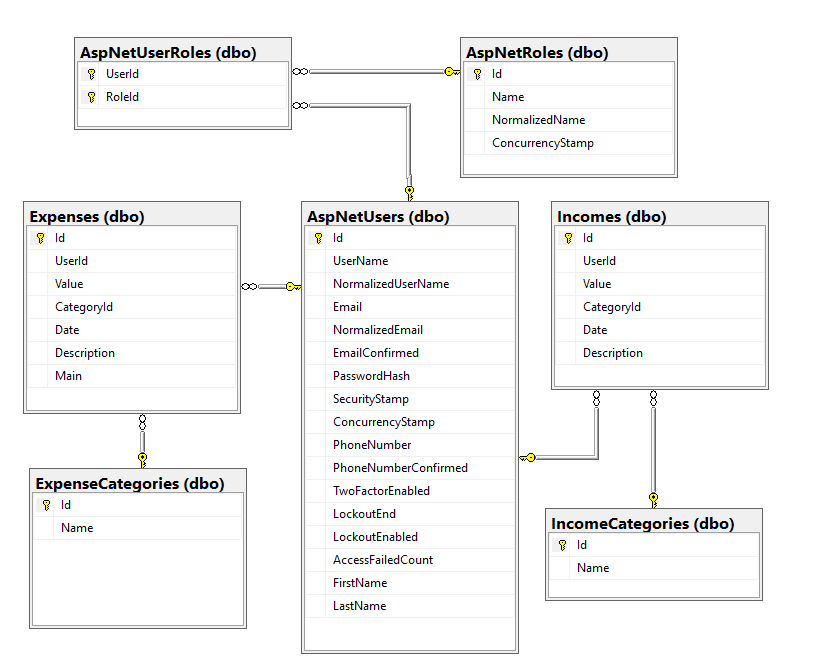
\includegraphics[width=6in]{img/diagram/db_diagram.png}
		\caption{Diagram bazy danych}
		\label{db_diagram}
	\end{center}
\end{figure}

Dostęp do danych w bazie danych z poziomu części serwerowej odbywa się przy pomocy klas encyjnych i mapowania relacyjno-obiektowego oraz klas zapewniających podstawowe operacje na danych. Diagram typów tej warstwy znajduje się na Rys. \ref{dal_dependecies}. Wszystkie klasy encyjne implementują interfejs \lstinline|IEntity| oraz odwzorowują strukturę bazy danych, a metody dostępu do danych dla pozostałych warstw aplikacji zapewnione są przez generyczny interfejs \lstinline|IApplicationRepository<TEntity>|, gdzie typ \lstinline|TEntity| obrazuje klasę encyjną (Rys. \ref{iapprepository}).\\
Dodatkowo w warstwie modelu danych znajduje się klasa \lstinline|DataInitializer|, która zawiera początkowe dane, jakie baza danych musi zawierać przy uruchomieniu aplikacji. Dane te są umieszczane w bazie podczas migracji, czyli procesu tworzącego strukturę bazy danych na podstawie istniejących klas encyjnych.
\begin{figure}[!ht]
\begin{center}
	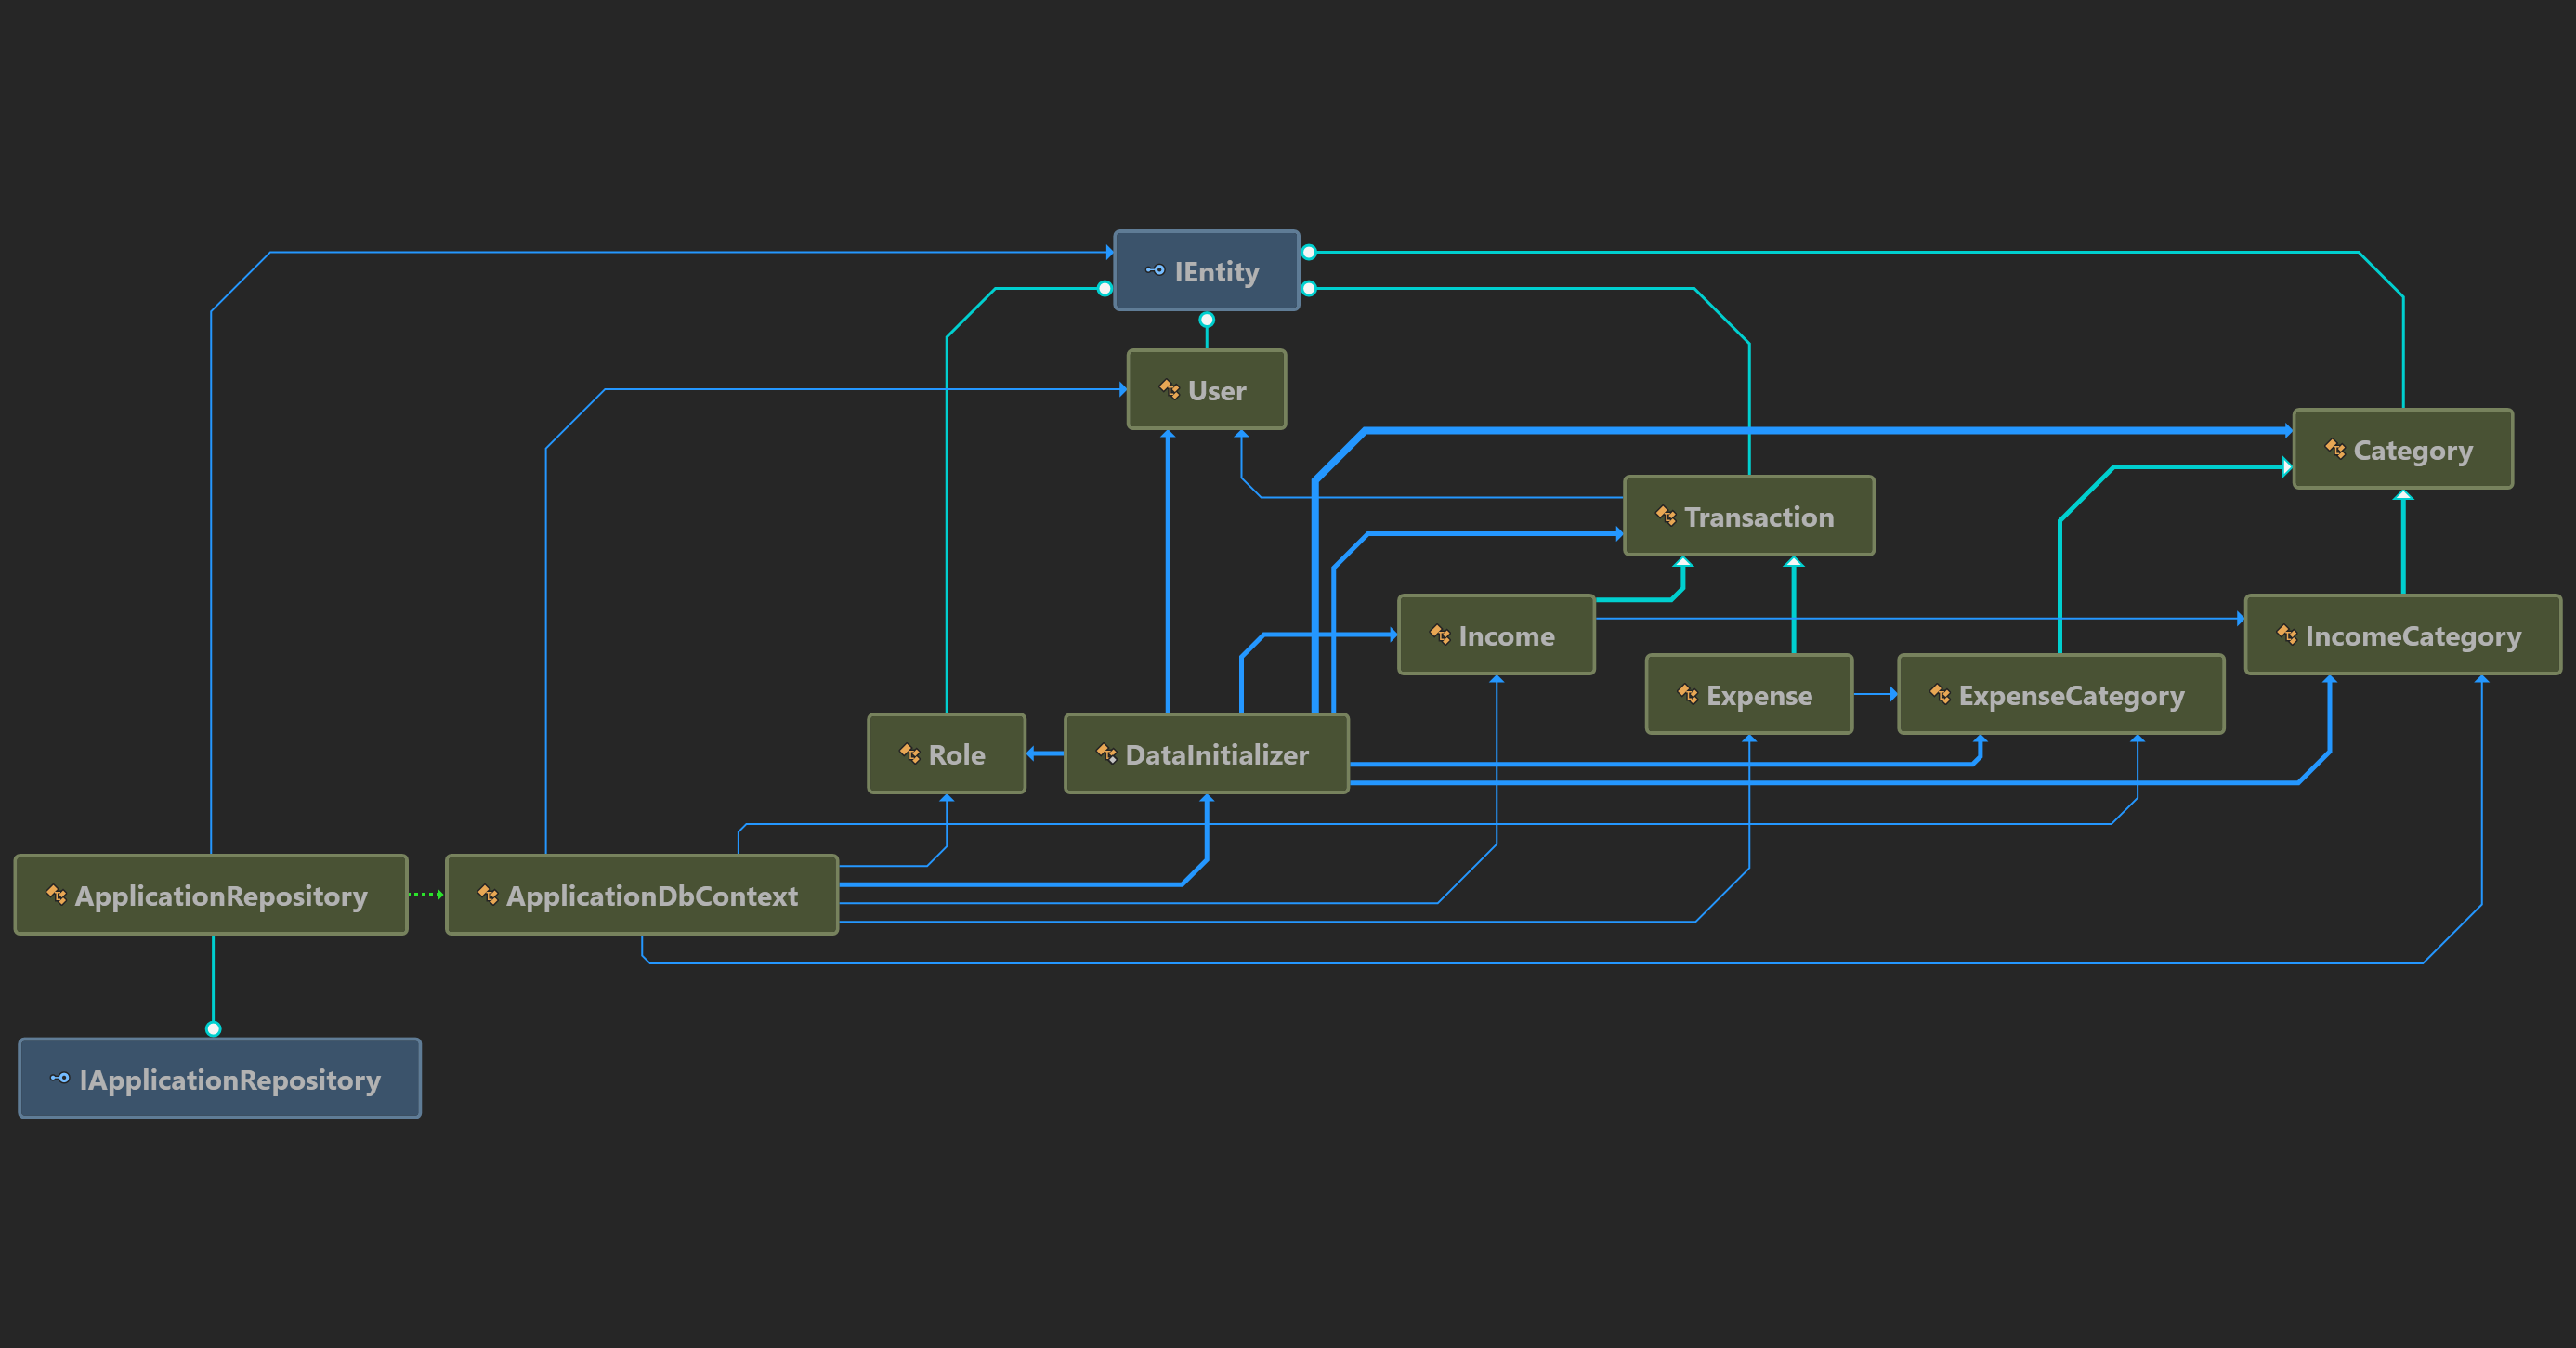
\includegraphics[width=6in]{img/diagram/dal_dependencies.png}
	\caption{Diagram zależności typów warstwy modelu danych}
	\label{dal_dependecies}
\end{center}
\end{figure}
\begin{figure}[!ht]
\begin{center}
	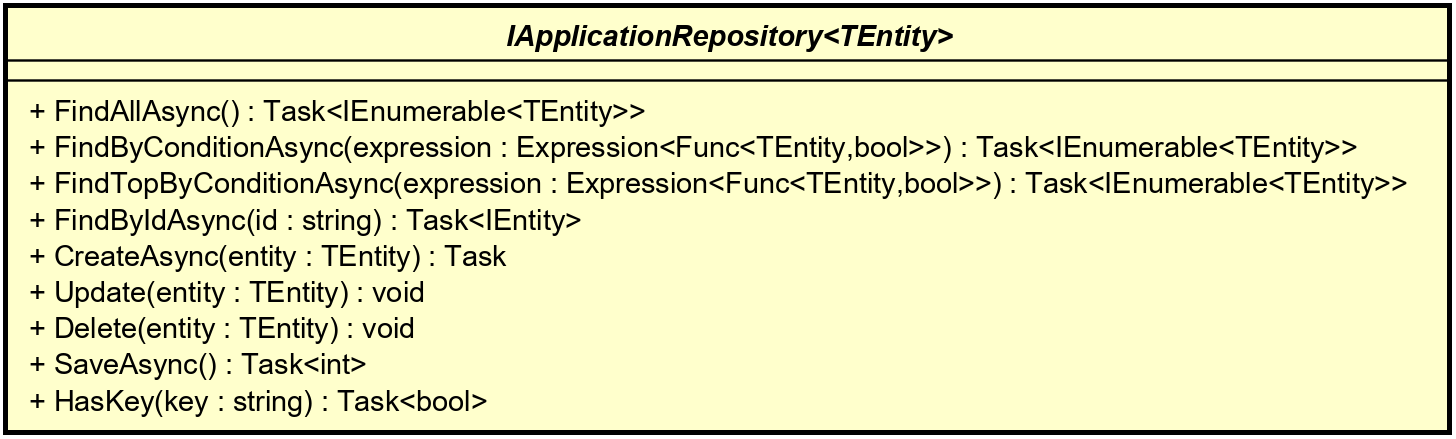
\includegraphics[width=6in]{img/diagram/iapprepository.png}
	\caption{Diagram interfejsu \lstinline|IApplicationRepository|}
	\label{iapprepository}
\end{center}
\end{figure}
\section{Warstwa logiki biznesowej}
Na warstwę logiki biznesowej składają się klasy realizujące logikę przypadków użycia, typy definiujące DTO i wyjątki aplikacyjne oraz klasy kontrolerów, pozwalających na dostęp do części serwerowej z poziomu aplikacji klienckiej.\\
W warstwie tej można wydzielić cztery moduły: moduł danych użytkownika, moduł wydatków, moduł przychodów oraz moduł predykcji. Moduły te mają podobną strukturę klas.\\
Na Rys. \ref{expensediagram} przedstawiony jest diagram zależności typów modułu wydatków. Klasa \lstinline|ExpenseController| odpowiedzialna jest za obsługę zapytań aplikacji klienckiej. Po otrzymaniu zapytania, klasa \lstinline|ExpenseService| implementująca interfejs \lstinline|IExpenseService| przy pomocy repozytorium znajdującego się w warstwie modelu danych obsługuje zapytanie użytkownika oraz zwraca jego wynik przy użyciu typu implementującego \lstinline|IDataTransferObject|. Mapowanie klasy encyjnej na typ DAO jest zdefiniowane w klasie \lstinline|MappingProfile|.
\begin{figure}[!ht]
	\begin{center}
		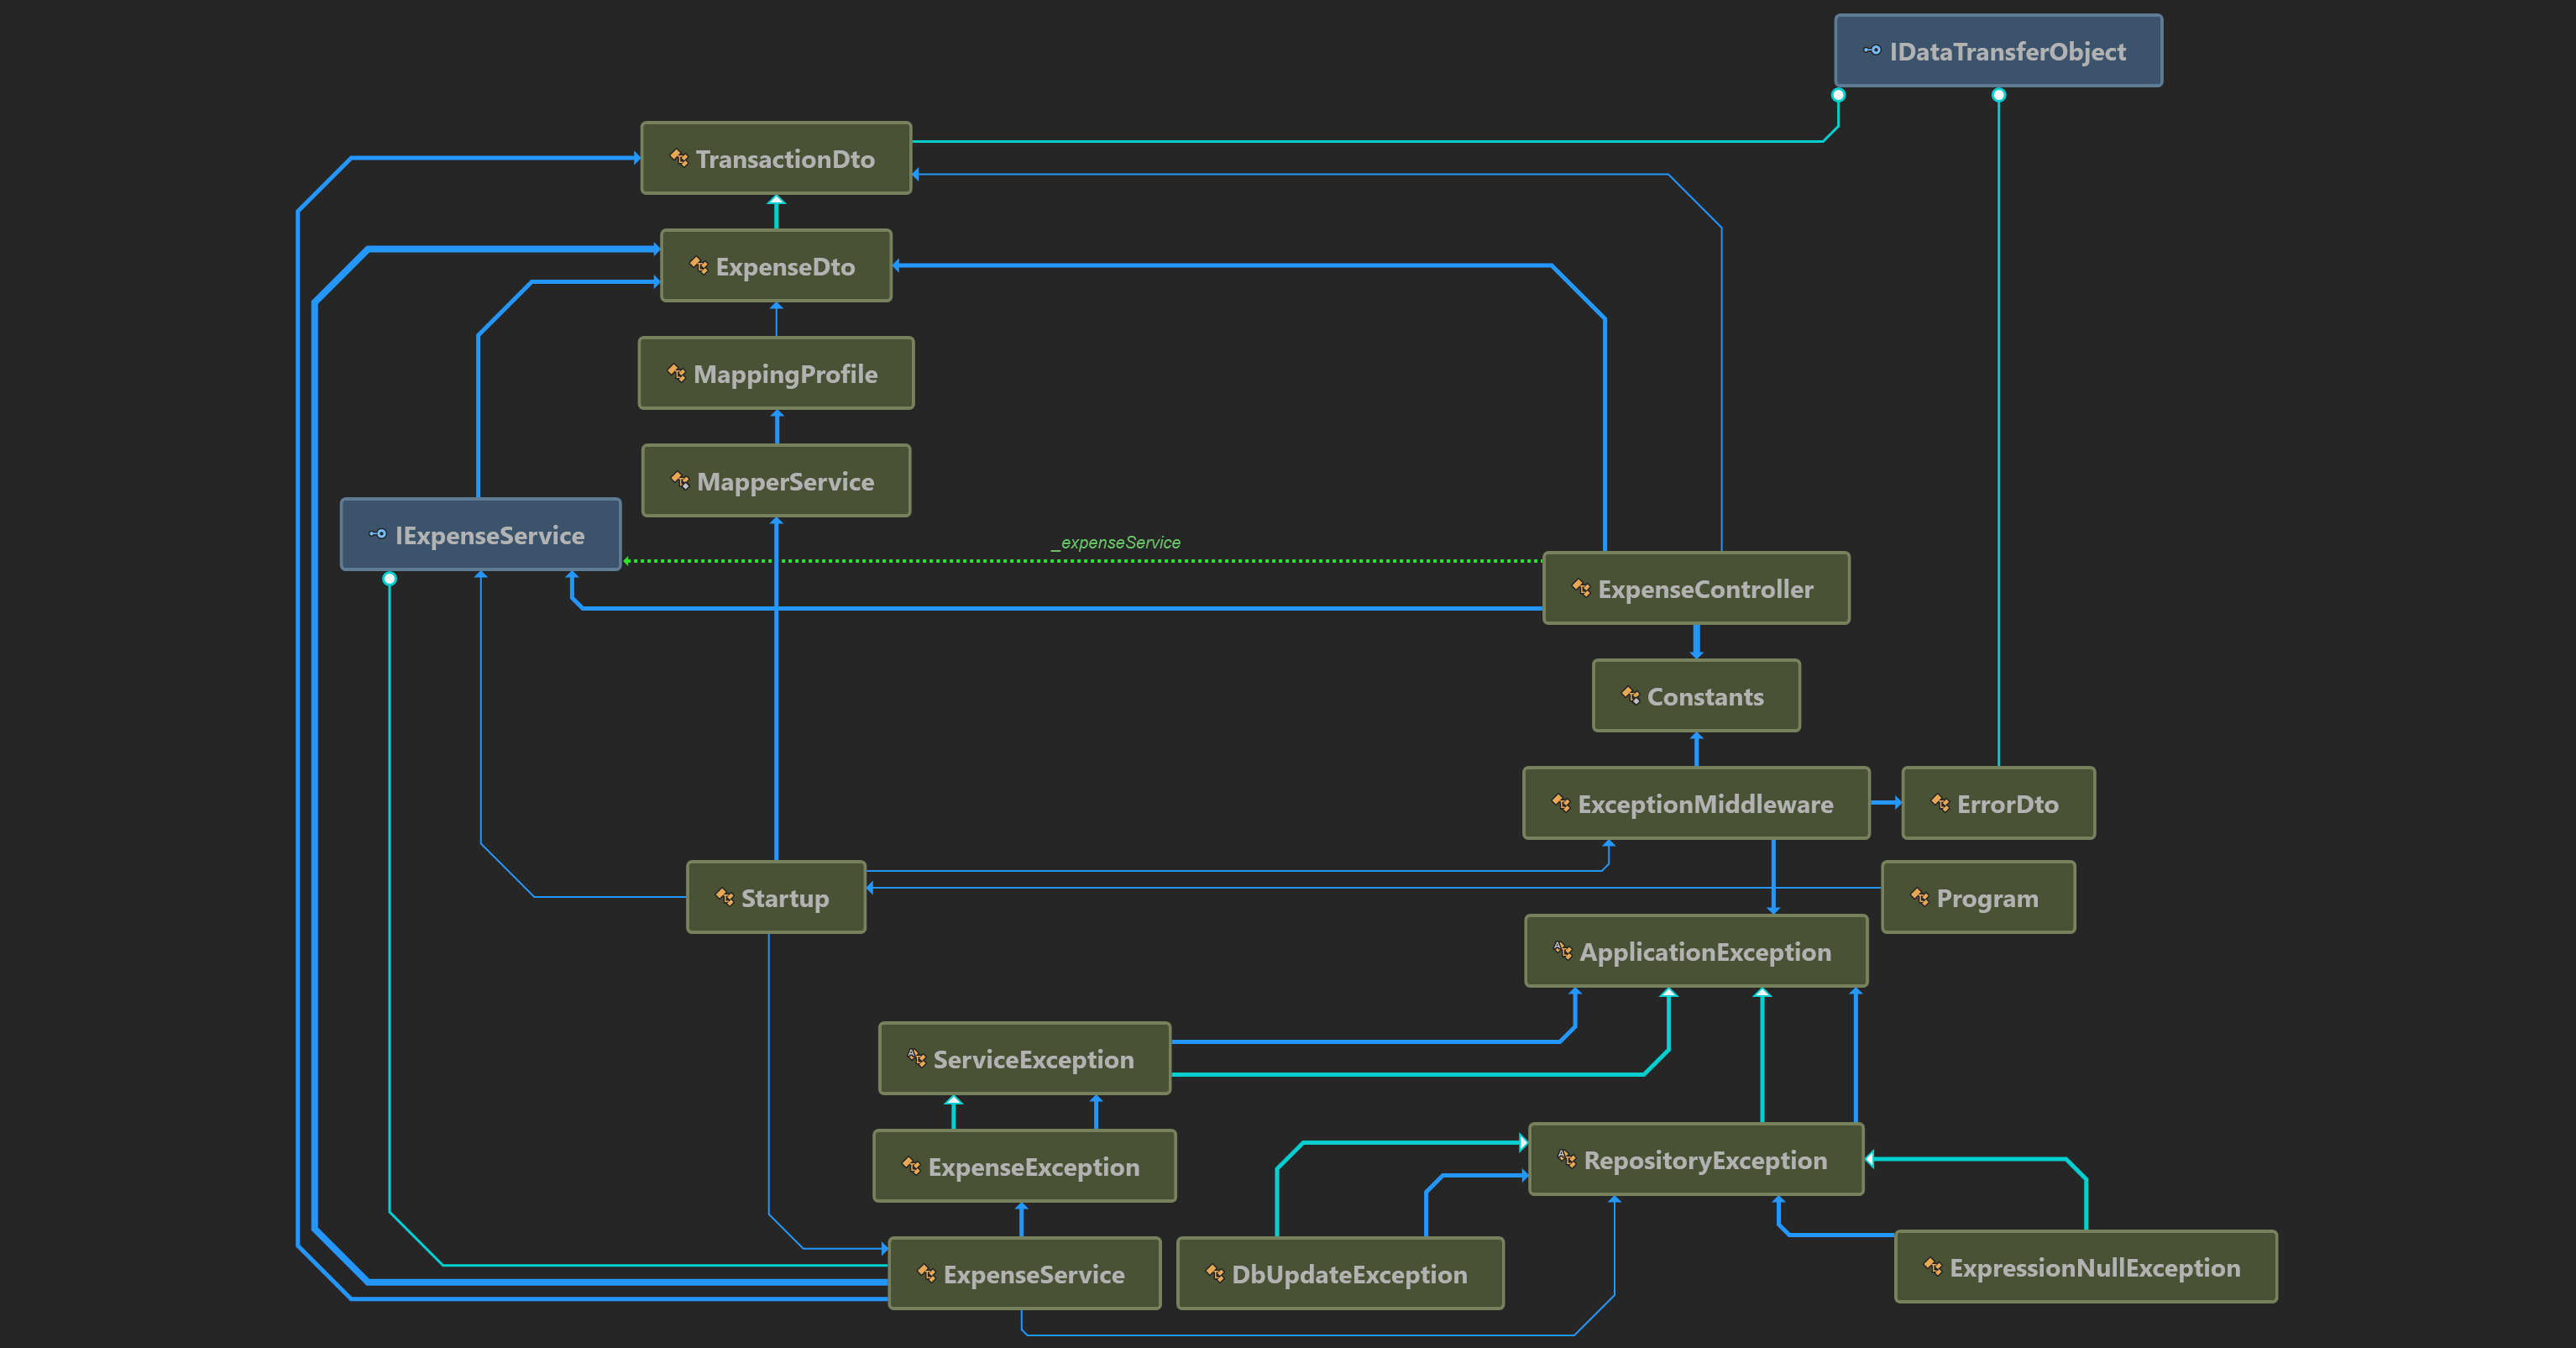
\includegraphics[width=6in]{img/diagram/expense_diagram.png}
		\caption{Diagram zależności typów warstwy logiki biznesowej dla modułu wydatków.}
		\label{expensediagram}
	\end{center}
\end{figure}
\section{Warstwa interfejsu użytkownika - aplikacja mobilna}